\documentclass{tufte-handout}

\title{Föreläsning 1: Permutationer och kombinationer $\cdot$ 1MA020}

\author[Vilhelm Agdur]{Vilhelm Agdur\thanks{\href{mailto:vilhelm.agdur@math.uu.se}{\nolinkurl{vilhelm.agdur@math.uu.se}}}}

\date{16 januari 2023}


%\geometry{showframe} % display margins for debugging page layout

\usepackage{graphicx} % allow embedded images
  \setkeys{Gin}{width=\linewidth,totalheight=\textheight,keepaspectratio}
  \graphicspath{{graphics/}} % set of paths to search for images
\usepackage{amsmath}  % extended mathematics
\usepackage{booktabs} % book-quality tables
\usepackage{units}    % non-stacked fractions and better unit spacing
\usepackage{multicol} % multiple column layout facilities
\usepackage{lipsum}   % filler text
\usepackage{fancyvrb} % extended verbatim environments
  \fvset{fontsize=\normalsize}% default font size for fancy-verbatim environments

\usepackage{color,soul} % Highlights for text

% Standardize command font styles and environments
\newcommand{\doccmd}[1]{\texttt{\textbackslash#1}}% command name -- adds backslash automatically
\newcommand{\docopt}[1]{\ensuremath{\langle}\textrm{\textit{#1}}\ensuremath{\rangle}}% optional command argument
\newcommand{\docarg}[1]{\textrm{\textit{#1}}}% (required) command argument
\newcommand{\docenv}[1]{\textsf{#1}}% environment name
\newcommand{\docpkg}[1]{\texttt{#1}}% package name
\newcommand{\doccls}[1]{\texttt{#1}}% document class name
\newcommand{\docclsopt}[1]{\texttt{#1}}% document class option name
\newenvironment{docspec}{\begin{quote}\noindent}{\end{quote}}% command specification environment

\include{mathcommands.extratex}

\begin{document}

\maketitle% this prints the handout title, author, and date

\begin{abstract}
\noindent
Vi börjar med att fråga oss vad kombinatorik ens är för något. Sedan introducerar vi några väldigt grundläggande begrepp och principer i ämnet, och tillämpar dem på att diskutera permutationer och kombinationer.
\end{abstract}

\section{Vad är kombinatorik?}

Jag hörde en gång, på en fest under min masterutbildning, en utläggning av en doktorand om att all matematik handlar om att reducera sina problem till en enklare form -- och i slutändan var alla matematikproblem antingen linjär algebra, i vilket fall de var lätta, eller så var de kombinatorik, i vilket fall de var svåra. Vi skall alltså studera den svåra delen av matematiken.

En annan överförenklande kategorisering av matematiken ges oss av Randall Munroe.\cite{XKCD_math_classification} Kombinatorik sysslar med den mellersta sortens problem -- där det är lätt att förstå frågan, och inga märkliga kontinuerliga objekt är involverade, men svaret ändå kan vara komplicerat att ta reda på.

\begin{figure}[h]
	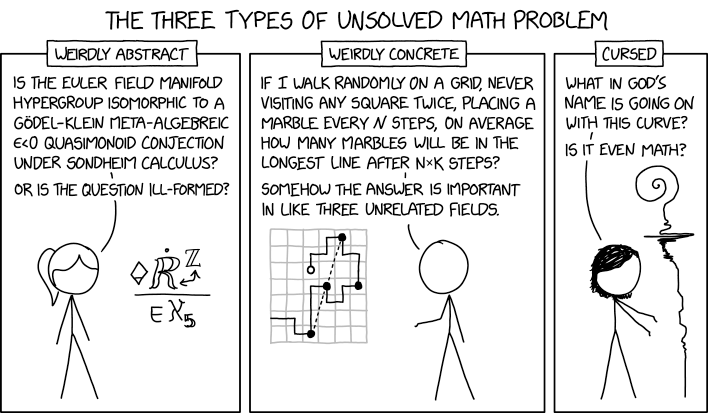
\includegraphics{graphics/unsolved_math_problems.png}
	%\caption{Tre typer av olösta matematikproblem}
\end{figure}

En mer ordboksmässig definition av vad kombinatorik är vore att säga att det handlar om att räkna saker, när sakerna är ändligt många och diskreta. Detta är dock heller ingen precis eller uttömmande definition, så det finns saker som är kombinatorik utan att nödvändigtvis handla om att räkna saker, till exempel inom grafteori.

\section{Varför studera kombinatorik?}

Kombinatorik har som redan nämnts tillämpningar i ren matematik -- många problem inom andra grenar av matematiken kan reduceras till problem i kombinatorik. Det har också otaliga tillämpningar utanför den rena matematiken:
\begin{enumerate}
	\item Nätverk och grafer
	\item Analys av algoritmer
	\item Design av kretskort
	\item Design av experiment
\end{enumerate}
Merparten av alla pussel-spel av typen sudoku, eller ``flytta bilarna för att få ut en specifik bil'', etc., kan ses som rena kombinatorikproblem.

\section{Additions- och multiplikations-reglerna}

\begin{definition}[Additions-regeln]
	Om $A$ är en mängd av $n$ objekt och $B$ är en mängd av $m$ objekt så finns det $n+m$ sätt att välja ett objekt från $A$ \emph{eller} ett objekt från $B$. Eller formulerat i symboler, om $\abs{A} = n$ och $\abs{B} = m$ så är $\abs{A \coprod B} = n + m$.\sidenote[][-1cm]{Symbolen $\coprod$ (Kan också skrivas som \uplus) betyder \emph{disjunkt union} -- vi tar unionen av de två mängderna, men vi tvingar mängderna att vara disjunkta genom att komma ihåg vilken mängd varje element kom från.  Så om $A$ och $B$ inte har några gemensamma element är det samma sak som $\cup$, men om de har gemensamma element gäller att t.ex. $\{1,2,3\}\cup \{3,4\} = \{1,2,3,4\}$, emedan $\{1,2,3\} \coprod \{3,4\} = \{(1,A), (2,A), (3,A), (3,B), (4, B)\}$, så de har alltså olika antal medlemmar.

För det allra mesta behöver man inte vara så här rigorös, men det kan vara bra att ha i bakhuvudet att summa-regeln inte räknar antalet element i $A\cup B$ om $A$ och $B$ kan tänkas ha gemensamma element. Vad vi gör i det fallet kommer vi återkomma till senare, när vi diskuterar inklusion-exklusion.}
\end{definition}

\begin{example}\label{example_addition_rule_with_cans}
    Vi har två burkar med olikfärgade kulor. Om vi ska plocka ut en kula från en av brukarna, på hur många sätt kan vi göra det?
\begin{figure}[h]   
    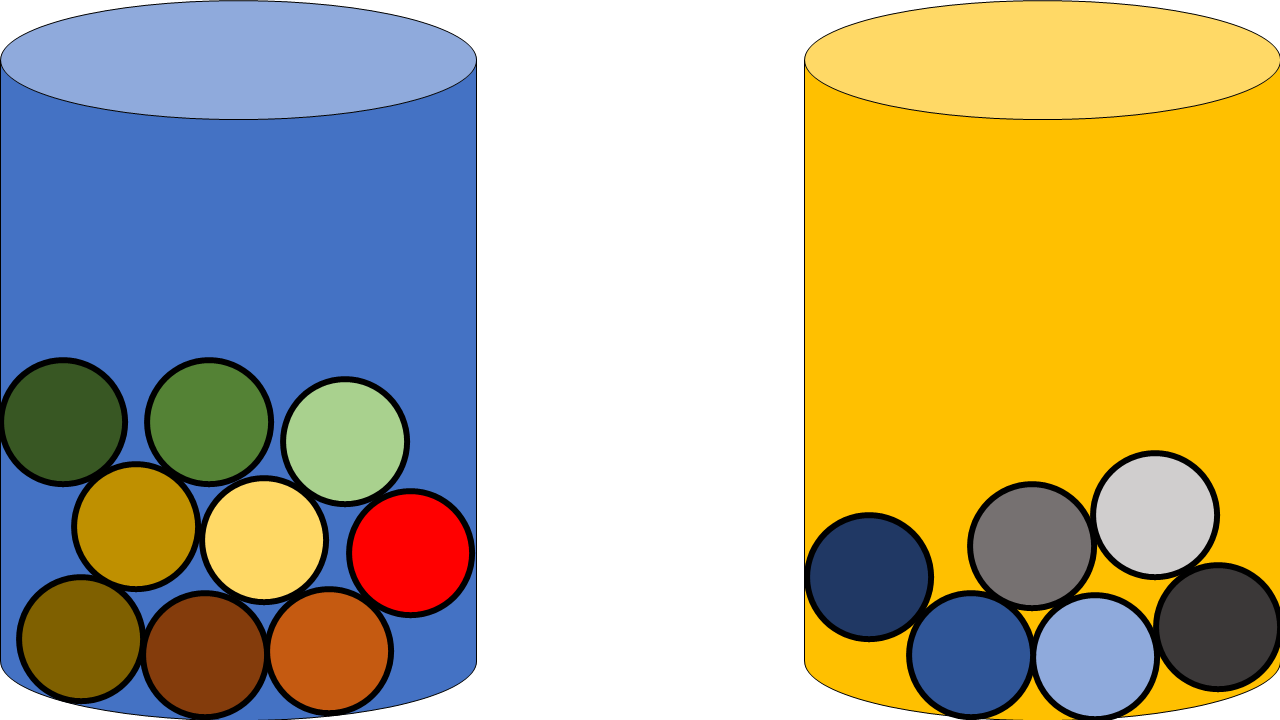
\includegraphics{graphics/burkar med kulor.png}
	%\caption{Två separata burkar med kulor i}
\end{figure}

    Vi kan använda additionsregeln för att beräkna det och det ges av $9+6=15$, vilket summerar antalet kulor totalt vi har att välja bland.
\end{example}

\begin{example}\label{example_addition_rule}
En restaurang har en meny med fyra drinkar, fem förrätter, tio huvudrätter, och tre desserter. Hur många saker har de på menyn?

Additions-regeln säger oss att svaret är $4+5+10+3 = 22$.
\end{example}

\begin{definition}[Multiplikations-regeln]
	Om $A$ är en mängd av $n$ objekt och $B$ är en mängd av $m$ objekt så finns det $nm$ sätt att välja ett objekt från $A$ \emph{och} ett objekt från $B$. Eller ekvivalent, det finns $nm$ sätt att välja ett par av ett objekt ur $A$ och ett objekt ur $B$. Eller uttryckt i symboler
$$\abs{A\times B} = \abs{\{(a,b) \given a \in A, b \in B\}} = nm.$$
\end{definition}

\begin{example}
    Om vi har samma två burkar som i Exempel \ref{example_addition_rule_with_cans}, på hur många sätt kan välja en kula från den blå burken och en kula från den gula burken?\\
    Med hjälp av bilden från Exempel\ref{example_addition_rule_with_cans} och multiplikationsregeln ger det oss att antalet olika sätt att välja två kulor, från en burk vardera, till $9\times 6 = 54$   
\end{example}

\begin{example}
	Om du besöker restaurangen i Exempel \ref{example_addition_rule}, hur många olika sätt finns det att beställa en trerätters middag med en drink till?
\sidenote{En fullständigt teoretisk fråga, eftersom ingen faktiskt har råd med det i dagens ekonomi.} Multiplikations-regeln säger oss att svaret är $4\times 5\times 10\times 3 = 600$.
\end{example}

\section{Strängar}

\begin{definition}
En \emph{sträng} $s$ (eller ett \emph{ord}) av längd $n$ på en mängd $X$ (kallad \emph{alfabetet} för strängen) är en funktion
$$s: \{1, 2, \ldots, n\} = [n] \to X$$
där $s_i$ är den $i$te bokstaven i ordet.\sidenote{Från och med nu kommer vi konsekvent använda notationen $[n]$ för mängden av tal mellan $1$ och $n$.}
Vi skriver detta oftast som $s = x_1x_2\ldots x_n$, där $x_i = s(i)$.
\end{definition}

\begin{example}[Binära strängar]
Låt $X = \{0,1\}$. Strängar $s: [n] \to X$ kallas för \emph{binära strängar}. Det finns $2^n$ strängar av längd $n$.\sidenote{Så det finns till exempel åtta binära strängar av längd tre, nämligen
$$000, 001, 010, 011, 100, 101, 110, 111.$$}

Hur vet vi detta? Det finns två val för varje bokstav, så multiplikationsregeln säger oss att det måste finnas $2\times 2\times\ldots\times 2 = 2^n$ att göra ett val av vad varje bokstav skall vara.
\end{example}

\begin{example}[$m$-ära strängar]
Låt $X = \{0,1,\ldots,m-1\}$. Strängar med detta alfabetet kallas för $m$-ära strängar. Om $m = 2$ är de binära, om $m = 3$ är de ternära. 
\end{example}

För generella $X$ kallar vi en sträng $s: [n] \to X$ för en $X$-sträng.

\section{Permutationer}

\begin{definition}
En sträng $s: [k] \to X$ kallas för en \emph{permutation} av längd $k$ av elementen i $X$ om alla bokstäverna i $s$ är olika, det vill säga om $s(i) \neq s(j)$ ifall $i \neq j$.
\end{definition}

Självklart måste $\abs{X} \geq k$ för att det skall existera några permutationer av längd $k$ av $X$.\sidenote{Hur hade du bevisat det?\\
Om vi antar att $\abs{X} < k$ men vi ska välja ut en permutation av längd k. Då börjar vi att välja ut första bokstaven $i_1$, sedan nästa bokstav $i_2$, och så vidare. Detta går bra tills vi har valt bokstav i X, låt oss kalla den $j$. Efter det har vi valt varje bokstav i alfabetet och kommer då behöva återanvända bokstäver i X. Men detta är inte tillåtet eftersom $s(i) \neq s(j) $ ifall $i \neq j$. Alltså kan vi inte skapa en perumatation av längd k om $\abs{X} < k$. Så $\abs{x} \geq k$}}

\begin{example}
Låt $X = [3]$. Det finns $6$ permutationer av längd $2$ av $X$\sidenote[][3.5cm]{Dessa är, specifikt, $$12, 13, 21, 23, 31, 32.$$} -- vi kan se detta med hjälp av multiplikationsprincipen: Vi har tre val av första bokstav, men när vi valt den har vi bara två val kvar av andra bokstav, eftersom vi inte får ha två av samma. Alltså är det totala antalet $3\times 2 = 6$.


\begin{center}
     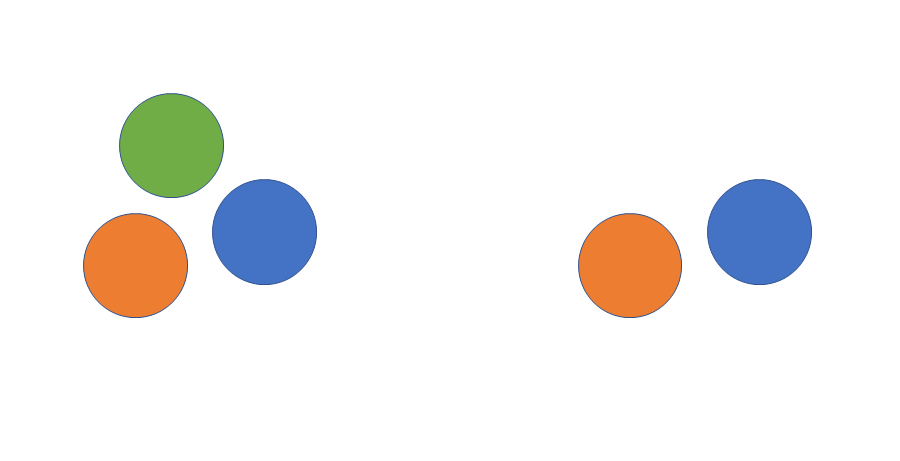
\includegraphics{graphics/bildpresentation.png}
\end{center}  

I bilden ser vi en representation av exempel 9. Tänk att de olika färgerna representerar olika bokstäver. Vi har från början tre bokstäver. Vi väljer först en bokstav och då har vi tre val, när vi valt en har vi två bokstäver kvar att välja på. 
\end{example}

\begin{definition}
För $n = 1, 2,\ldots$, definiera $n! = n\times(n-1)\times\ldots\times2\times1$. Definiera $0! = 1$.\sidenote{Att vi låter $0!$ vara lika med ett är för att vi ser det som produkten av inga tal alls, vilket är bekvämt att se som att det blir $1$. Varför detta är så kommer vi kanske att återkomma till när vi pratar om rekursioner.}

För $k \leq n$, definiera $P(n,k) = \frac{n!}{(n-k)!}$. Lägg märke till att $P(n,n) = \frac{n!}{(n-n)!} = \frac{n!}{0!} = n!$.
\end{definition}

\begin{proposition}\label{prop_Pnk_counts_permutations}
Om $\abs{X}=n$ och $0 \leq k \leq n$ så finns det $P(n,k)$ permutationer av längd $k$ från $X$.
\begin{proof}
Vi bevisar detta med hjälp av multiplikationsprincipen -- så vi skall räkna hur många sätt vi kan välja vår permutation $x_1x_2\ldots x_k$ på. Det finns så klart $\abs{X} = n$ sätt att välja första bokstaven $x_1$ i vår permutation. När vi sedan skall välja $x_2$ får den inte vara lika med $x_1$, så vi väljer ett element ur $X \setminus \{x_1\}$, och $\abs{X\setminus\{x_1\}} = n-1$. Likaledes för $x_3$ så får den varken vara lika med $x_1$ eller $x_2$, så vi väljer från $X\setminus \{x_1, x_2\}$, och har $n-2$ val.

Den här processen fortsätter tills vi skall välja $x_k$, och i det skedet har vi tagit bort $k-1$ val, och har alltså $\abs{X \setminus \{x_1, x_2, \ldots, x_{k-1}\}} = n - (k-1)$ bokstäver kvar att välja på.

Multiplikationsregeln säger oss att det totala antalet permutationer är lika med produkten av antalet val vi hade i varje steg, det vill säga
\begin{align*}
	n\cdot(n-1)\cdot(n-2)\cdot\ldots\cdot(n-(k-1)) &= \frac{n\cdot(n-1)\cdot(n-2)\cdot\ldots\cdot2\cdot1}{(n-k)\cdot\ldots\cdot2\cdot1}\\
	&= \frac{n!}{(n-k)!} = P(n,k).
\end{align*}
\end{proof}
\end{proposition}

\begin{example}
	På hur många olika sätt kan $n$ personer sitta runt ett runt bord?\sidenote{Det finns en liten ritning av detta i anteckningarna från föregående år, och jag lär rita den på den faktiska föreläsningen.}

	Det finns två olika sätt vi kan se på frågan\sidenote{Detta är ett exempel av skillnaden mellan problem med etiketter och utan, vilket är ett generellt fenomen som kommer återkomma gång på gång. Här är det platserna runt bordet som kan ha etiketter eller inte. Var noggrann med att fundera kring vilken typ av } -- antingen är det skillnad på de olika stolarna runt bordet (vissa kan se ut genom fönstret, andra inte), så att vi får olika sätt att placera folk runt bordet genom att rotera hela placeringen, eller så är det enda som spelar roll ordningen de sitter i, och vi ser olika rotationer av samma ordning som samma sätt att sitta runt bordet.

	Om platserna har etiketter, så att det inte bara är ordningen som spelar roll, så kan vi numrera platserna från plats $1$ till plats $n$. Om vi kallar mängden med gäster för $X$ blir alltså varje placering ett $X$-ord -- vi kan skriva den som ``gäst ett, gäst två, etc.''. Och eftersom varje person bara kan sitta på en stol blir detta alltså en permutation -- och vi vet att det finns $n!$ permutationer av längd $n$ ur ett alfabete med $n$ bokstäver.
 
\begin{center}
    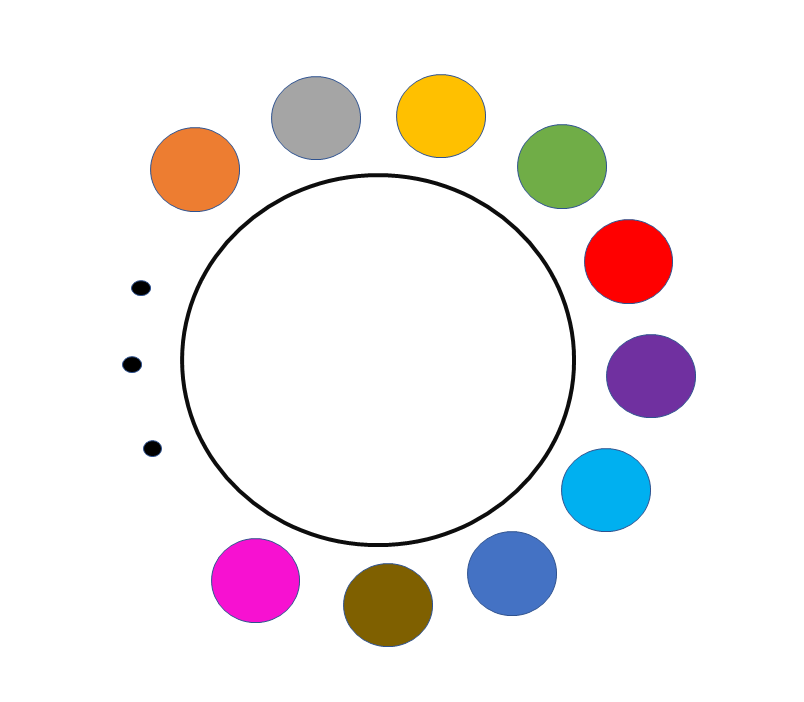
\includegraphics[width=0.7\textwidth]{graphics/bordmedfarg1.png}
\end{center}


        Bilden ovan visar de olika platserna och de olika platserna har olika färger. Vi kan då se det som att det inte är samma sak att sitta på en blå pall som att sitta på en orange pall tillexempel. Alltså kommer då spela roll vilken stol man sitter på och vem man sitter brevid. \sidenote{De svmå svarta pickarna beskriver att det finns många fler platser, så att summan blir n stycken platser.}

	Om platserna är oetiketterade, det vill säga att det enda vi bryr oss om är ordningen folk sitter i, får vi räkna på ett annat sätt. Givet en placering kan vi godtyckligt välja en person som ``först'', och sedan numrera platserna i medurs ordning. För varje av de $n$ sätten att välja vem som är först får vi alltså en placering där platserna har etiketter.

	Detta ger oss ett annat sätt att räkna antalet placeringar med etiketter -- vi räknar antalet utan etiketter, kallar det $m$, och får alltså att antalet med etiketter är $nm$.

	Men eftersom vi redan vet att antalet när platserna har etiketter är $n!$ så får vi alltså av detta att $n! = nm$, eller $m = \frac{n!}{n} = (n-1)!$, och vi har räknat antalet utan etiketter till $(n-1)!$.\sidenote{Detta är ett vanligt sätt att resonera inom kombinatorik -- vi hittade två olika sätt att räkna samma sak, och fick på så sätt ut en likhet ($nm = n!$) som vi kunde använda för att räkna en annan sak.}
 
 \begin{center}
      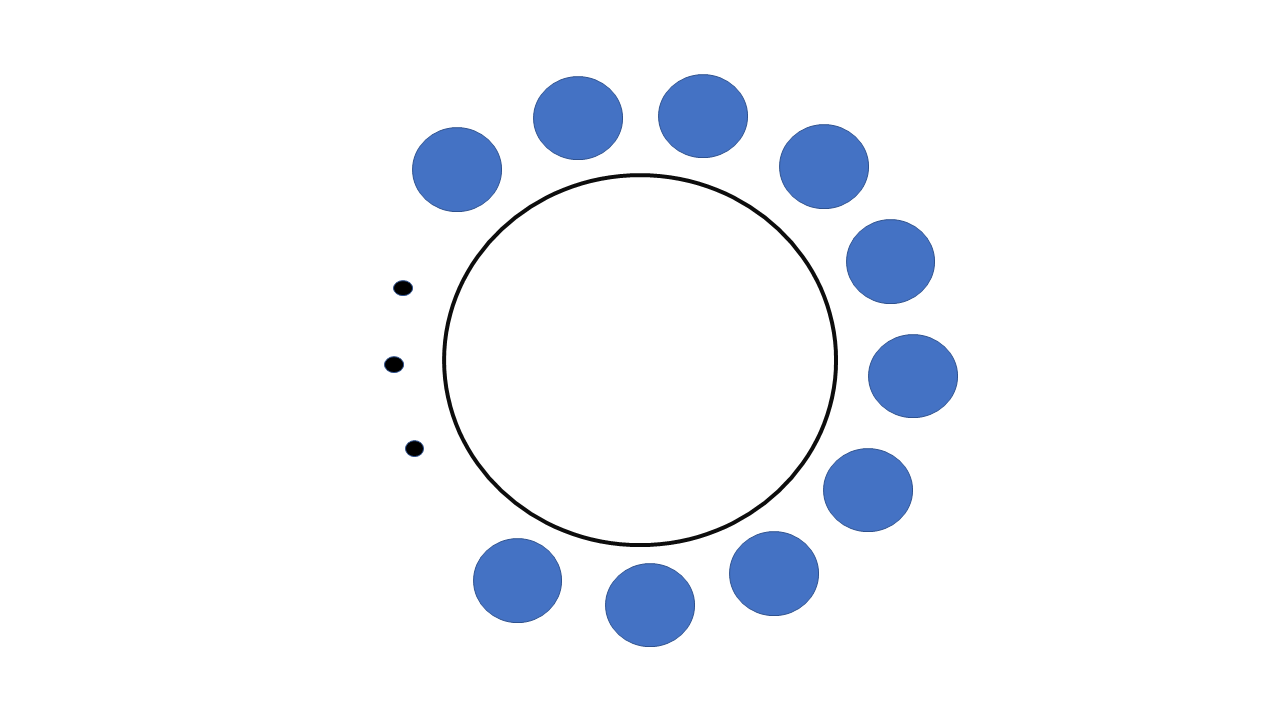
\includegraphics[width=0.9\textwidth]{graphics/bordutanfarg1.png}
 \end{center}

       Här är alltså varje plats likadan och det kommer endast spela roll vem man sitter brevid, till skillnad från vid förra bordet. Se figur \ref{fig:4}. \sidenote{De svmå svarta pickarna beskriver att det finns många fler platser, så att summan blir n stycken platser.} 
\end{example}
\section{Kombinationer}

\begin{definition}
	För en mängd $X$ så är en \emph{kombination} av element ur $X$ en delmängd $A \subseteq X$.\sidenote{Vi talade innan om etiketter och inte. Man kan se en kombination som en permutation utan etiketter -- vi vet bara vilka element som är med, inte i vilken ordning de kommer.}
\end{definition}

\begin{example}
	Det finns $6$ kombinationer av storlek $2$ från $X = \{a,b,c,d\}$, nämligen
	$$\{a,b\}, \{a,c\},\{a,d\},\{b,c\},\{b,d\},\{c,d\}.$$
\end{example}

\begin{definition}
	För $0 \leq k \leq n$, låt $\binom{n}{k} = \frac{P(n,k)}{k!} = \frac{n!}{k!(n-k)!}$. Man ser också notationerna $C(n,k)$, $nCk$, eller $C^n_k$ för detta, men vi håller oss till $\binom{n}{k}$. 
\end{definition}

\begin{proposition}
	Om $\abs{X} = n$ och $0 \leq k \leq n$ så finns det $\binom{n}{k}$ kombinationer av storlek $k$ från $X$.
	\begin{proof}
		Även detta bevisar vi med ``räkna på två olika sätt''-metoden. Låt oss börja med att räkna antalet \emph{permutationer} igen, på ett annat sätt än vi gjorde i beviset av Proposition \ref{prop_Pnk_counts_permutations}.

		Istället för att tänka oss att vi väljer en bokstav i taget, kan vi tänka oss att vi först väljer en mängd $A$ av bokstaver som skall vara med -- och då måste ju $\abs{A} = k$ eftersom varje bokstav skall dyka upp exakt en gång -- och sedan väljer en ordning i vilken bokstäverna skall dyka upp.

		Antalet sätt att välja en ordning för våra $k$ bokstäver är precis antalet permutationer av längd $k$ från alfabetet $A$, vilket vi vet är $P(k,k)$. Så om vi betecknar antalet sätt att välja mängden $A$ med $m$, så säger oss multiplikationsregeln att antalet permutationer av längd $k$ från $X$ måste vara $m\cdot P(k,k)$.

		Men vi vet ju också, från hur vi räknade antalet permutationer innan, att $P(n,k) = \frac{n!}{(n-k)!}$ och $P(k,k) = k!$. Så vad vi har visat är att
		$$\frac{n!}{(n-k)!} = P(n,k) = m P(k,k) = m k!$$
		eller, om vi löser för $m$, att
		$$m = \frac{n!}{k!(n-k)!}$$
		vilket är vad vi ville bevisa.
	\end{proof}
\end{proposition}

\begin{proposition}
	För alla $n \geq 0$ och alla $0 \leq k \leq n$ gäller det att
	$$\binom{n}{k} = \binom{n}{n-k}.$$
\end{proposition}

Vi ger två olika bevis av denna proposition. Det första är algebraiskt:
\begin{proof}
	\begin{align*}
		\binom{n}{k} &= \frac{n!}{k!(n-k)!}\\
		&= \frac{n!}{(n-(n-k))!(n-k)!}\\
		&= \frac{n!}{(n-k)!(n-(n-k))!} = \binom{n}{n-k}.
	\end{align*}
\end{proof}

Det andra är kombinatoriskt:\sidenote{Vad menar vi när vi säger att det här beviset är ``kombinatoriskt'', till skillnad från det andra beviset? Nyckeln är att vi här visade att de två mängderna -- mängden av delmängder av storlek $k$ och mängden av delmängder av storlek $n-k$ -- har lika många medlemmar genom att uppvisa en bijektion mellan dem, emedan vi i det algebraiska beviset bara manipulerade våra formler för att visa att de var lika.

Bijektionen vi hittade här är själv ett \emph{kombinatoriskt} objekt, och det berättar mer för oss än bara att mängderna har lika många medlemmar. Man kan se det som att den är en \emph{anledning} till varför de har lika många mängder.

Denna bevismetod, att hitta en bijektion, kommer vara ett återkommande tema -- och likaså att bijektionerna ger oss mer förståelse för objekten vi studerar än vad ett algebraiskt bevis gör.}
\begin{proof}
	Låt $X$ vara en mängd med $n$ element. $\binom{n}{k}$ räknar antalet sätt att välja en delmängd $A \subseteq X$ av storlek $k$. Men varje sådan delmängd $A$ har ett komplement $X\setminus A$ av storlek $n-k$, och för varje delmängd av storlek $n-k$ kan vi få en av storlek $k$ genom att ta dess komplement.

	Delmängder av storlek $k$ och delmängder av storlek $n-k$ står alltså i ett-till-ett-korrespondens med varandra, det finns en bijektion mellan dem, så det måste finnas lika många av storlek $k$ som av storlek $n-k$.

	Men vi vet att antalet delmängder av storlek $n-$ är $\binom{n}{n-k}$, och alltså måste $\binom{n}{k} = \binom{n}{n-k}$.

\end{proof}

 På bilderna nedan kan vi se två olika representationer av komplementet för k och k. 
 
\begin{center}
    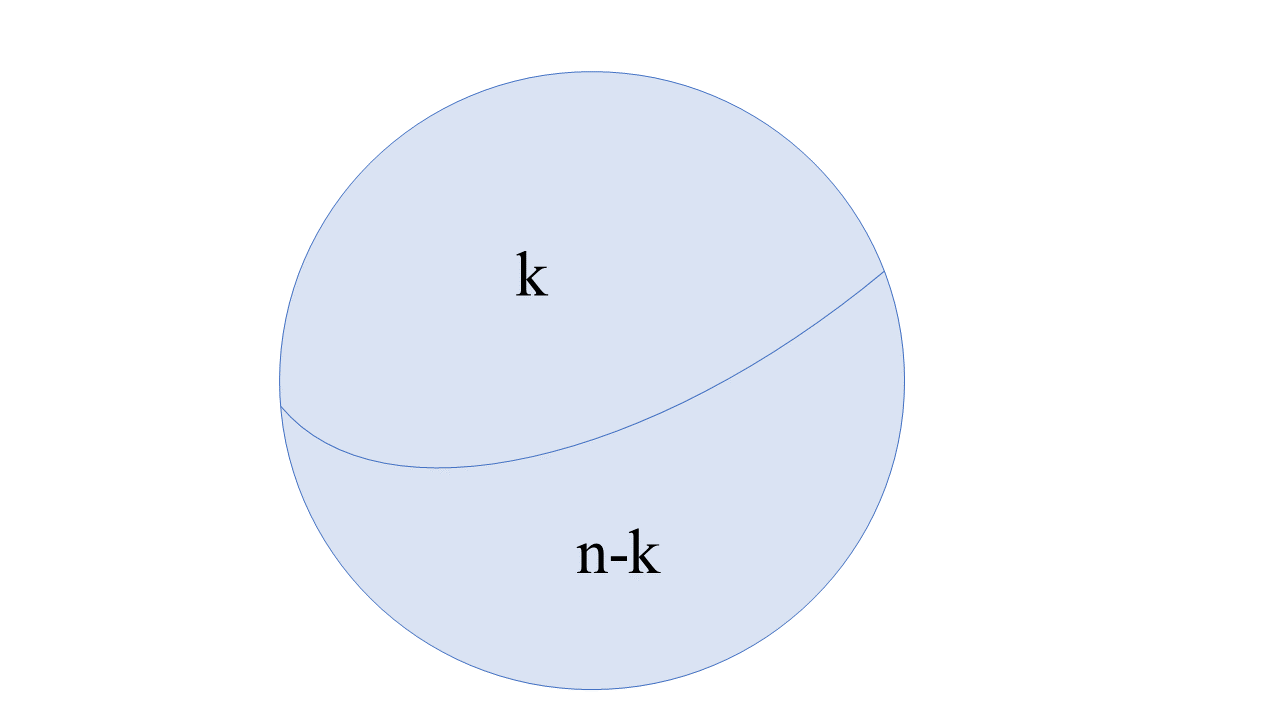
\includegraphics[width=0.7\textwidth]{graphics/komplementbild1.png}
\end{center}

\begin{center}
    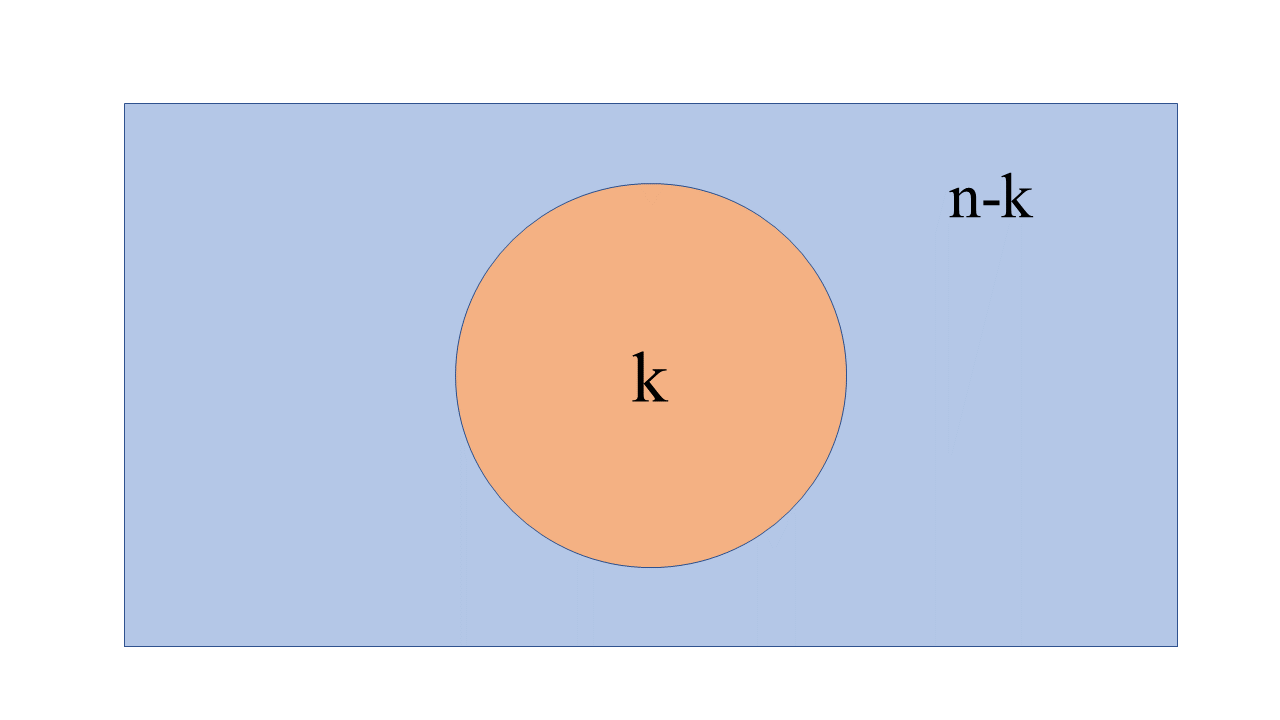
\includegraphics[width=0.7\textwidth]{graphics/komplementbild2.png}
 \end{center}

\bibliography{references}
\bibliographystyle{plainnat}

\section{Övningar}

\begin{xca}
	Tjugofyra studenter ska sitta vid ett långt bord\sidenote[][1cm]{Ni slipper alltså runda bord i denna övningen! Bordet har en första plats, en andra plats, och så vidare till tjugofjärde platsen.} och skriva en tenta. Tio av dem är väldigt benägna att fuska genom att kolla på sin kompis tenta.

	Deras kombinatoriklärare bestämmer att dessa tio studenter måste sitta på platser med udda nummer, så att de inte kan hamna bredvid varandra och fuska.

	Hur många sätt finns det att placera studenterna vid bordet?
\addlinespace
    \noindent\textbf{Lösning} 
    Vi börjar med att rita upp en bild för situationen.
\begin{center}
    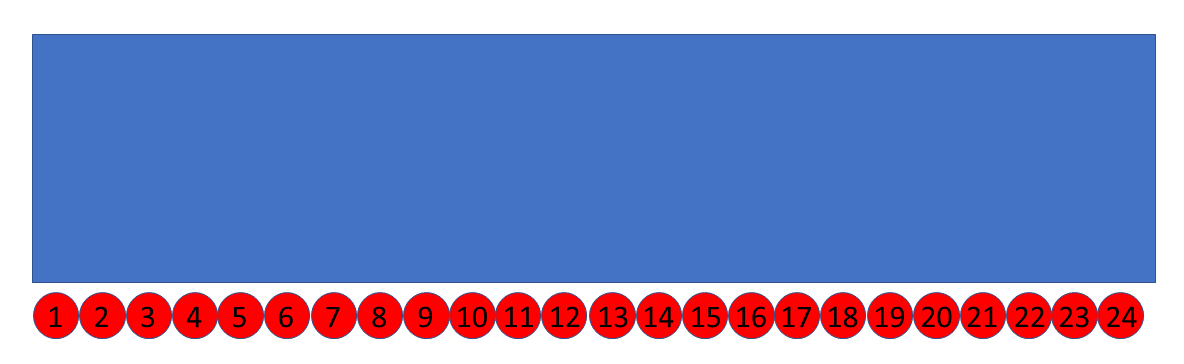
\includegraphics{bordmedstolar.png}
\end{center}
    Enligt uppgiften behöver vi placera ut de fuskande eleverna på udda stolsplatser, alltså ska vi placera ut 10 elever på 12 platser. Detta kan göras på $P(12,10)$ sätt. Därefter har vi 14 elever kvar att placeras ut på de kvarvarande 14 platserna. Det kan göras på $P(14,14)$ sätt. Det totala antalet sättet att placera ut alla elever blir därmed:\\
    $P(12,10)*P(14,14)=\frac{12!\cdot14!}{2!}$\\
    \noindent Anledningen till att vi använder permutationer i lösningen är för att vi ser stolsplatserna som unika.\\
    \noindent\textbf{Tips}
    Viktigt i liknande uppgifter är att identifiera ifall platserna, stolarna i det här fallet, är unika eller inte. Om det är unika, som i det här fallet, så använder vi oss av permutationer. Är det inte unika så får vi använda oss av kombinationer istället. Detta försöktes tydliggöras genom att numrerar stolsplatserna. 
    Ett sätt att enklare förstå uppgiften är att vi ska dela ut stolsnummer till eleverna, istället för att placera ut eleverna på stolarna. Då kan det bli enklare att förstå varför det går att placera ut de 10 fuskande eleverna på de 12 udda platserna blir $P(12,10)$. 12 stolsnummer ska delas ut till 10 personer
\end{xca}
\end{xca}

\begin{xca}
	Ge ett algebraiskt bevis för att
	$$k\binom{n}{k} = n \binom{n-1}{k-1}.$$
\end{xca}

\noindent\textbf{Lösning}
    $$HL = n \binom{n-1}{k-1} = \frac{n(n-1)!}{(k-1)!(n-1-(k-1))!}$$ $$= \frac{n(n-1)!}{(k-1)!(n-k)!} = \frac{k\cdot n!}{k!(n-k)!} = k\binom{n}{k} = VL$$
    
\noindent\textbf{Tips}
    Expandera utrycket genom att använda definitionen av binomialkoefficienter
    $$\binom{n}{k} = \frac{n!}{k!(n-k)!}$$
    Tänk på att n-fakultet kan skrivas som
    $$n! = n(n-1)(n-2)...2\cdot 1$$ 
    och att
    $$\frac{n}{n!} = \frac{1}{(n-1)!}$$

\begin{xca}
	Ge ett kombinatoriskt bevis för att\sidenote[][]{Ledtråd: Tänk på att välja grupper med ledare för ett projekt.}
	$$k\binom{n}{k} = n \binom{n-1}{k-1}.$$

    Från fotnoten får vi tipset att tänka på det som att välja en grupp med ledare. Vi försöker nu studera vänsterledet för sig och högerledet för sig för att kombinatoriskt bevisa likheten. 
        Vi kollar på vänsterledet först: Vi vill välja en grupp med k personer i och vi har totalt n stycken personer att välja på. För att få antalet sätt vi kan skapa denna gruppen tar vi $$\binom{n}{k}.$$. Nu har vi alltså beräknat antalet sätt att skapa en grupp med k personer. Nu vill vi välja en ledare bland dessa personer. Vi har då k potentiella ledare. Så För att beräkna antalet sätt vi kan skapa en grupp med k personer varav en person är ledare får vi då $$k\binom{n}{k}$$
        Nu tittar vi på högerledet: Vi vill visa att högerledet också beräknar antalet sätt att skapa en grupp med k personer varav en person är ledare. Vi har n personer att välja på och vi ska ha en grupp på k personer och en av de ska vara ledare. Nu börjar vi med att välja en person som ska vara vår ledare, vi har då n personer att välja på för att vara ledare. Nu vill vi välja en grupp till den här ledaren. Vi har n-1 personer kvar att välja på och k-1 platser kvar att fylla upp i gruppen. Antalet sätt att skapa gruppen av resterande personer blir då $$\binom{n-1}{k-1}.$$. Så antalet sätt att skapa en grupp med en ledare och k-1 medlemmar (alltså totalt k medlemmar) är då $$n \binom{n-1}{k-1}.$$. 
\end{proof}
\noindent\textbf{Tips}

         1. I denna uppgiften använde vi oss av att vi ska skapa grupper. Ett bra sätt att lösa liknande uppgifter är att se det som att vi ska skapa grupper med personer av olika slag. Det kan vara en grupp med en eller flera ledare, grupper av olika storlekar med olika många personer som ska väljas ut eller plockas bort med mera. Försök att skapa ett sammanhang.
         
         2. Är det svårt att hitta ett sammanhang så försök att identifiera variablerna en efter en, så i detta fallet försök först att identifiera vad k skulle kunna innebära och vad $$\binom{n}{k}$$ skulle kunna innebära. Försök också att starta med en sida, så antigen vänsterled eller högerled. Identifiera de olika variablerna (tillexdempel i ett sammanhang) på den sidan och försök sedan ska en matchning med andra sidan.
\end{xca}

\begin{xca}
	Ge ett kombinatoriskt bevis för att
	$$\binom{n}{2}\binom{n-2}{k-2} = \binom{n}{k}\binom{k}{2}.$$
	
\noindent\textbf{Lösning}
\begin{proof}
Här kan vi tänka på ungefär samma sätt som uppgift 3, men nu är skillnaden att vi ska välja 2 ledare istället för en. 
Vi Har en grupp på en personer och vi vill välja ut en liten grupp med k personer i varav 2 av de kommer utses till ledare. 
Vi börjar med vänsterledet: Vi har alltså n personer och vi vill välja två stycken ledare av alla de n personerna. Detta kan vi göra på $$\binom{n}{2}$$ sätt. När det är gjort så har vi n-2 personer kvar som inte blivit valda och av de n-2 personerna vill vi välja ut k-2 stycken för att skapa en grupp med k-2 personer och som tillsammans med ledarna skapar en grupp på k personer. Gruppen på k-2 personer kan vi skapa på $\binom{n-2}{k-2}$ sätt, eftersom vi har n-2 personer kvar. När vi då multiplicerar $$\binom{n}{2}\binom{n-2}{k-2}$$ får vi alltså antalet sätt att forma en grupp med k personer varav 2 stycken är ledare. 

Vi kollar på högerledet: I högerledet tänker vi först att vi vill skapa en grupp med k personer av de n stycken möjliga personerna. Antalet sätt att göra detta på är $\binom{n}{k}$. Så när vi har skapat en grupp med k personer i så vill vi välja två stycken ledare. Detta kan vi göra på $$\binom{k}{2}.$$ sätt eftersom vi har k stycken möjliga ledare och vi ska välja ut två stycken. 

Nu har vi visat att både vänsterledet och högerledet båda beräknar antalet sätt att forma en grupp med k personer i varav två personer är ledare. 
\end{proof}
\noindent\textbf{Tips}

Tipsen i denna uppgiften är samma som för uppgift 3. 

\end{xca}

\begin{xca}
	Antag att du har två mängder $A$ och $B$, med $\abs{A} = 15$ och $\abs{B} = 7$.
	\begin{enumerate}
		\item Hur många sätt finns det att välja ett objekt från $A$ eller ett från $B$?
		\item Hur många sätt finns det att välja ett objekt från $A$ och ett från $B$?
		\item Vad är $\abs{A\times B}$?
		\item Vad är $\abs{A \coprod B}$?
		\item Vad är det största och minsta värde som $A \cup B$ kan ta?
		\item Vad är det största och minsta värde som $A \cap B$ kan ta?
	\end{enumerate}

 \noindent\textbf{Lösning}

 \addlinespace 
 
 1. Det finns $\abs{A} + \abs{B} = 15 + 7 = 22$. stycken sätt att välja ett objekt från A eller ett objekt från B. Detta gäller från additionsregeln.
 
\addlinespace

 2. Det finns $\abs{A}\abs{B}  = 15 \cdot 7= 105$ sätt att välja ett objekt från A och ett objekt från B. Detta gäller från multiplikationsregeln. 
 
 \addlinespace

 3. Det är antalet sätt vi kan välja ett objekt ur A och ett objekt ur B, alltså $15 \cdot 7=105$. 

 \addlinespace

 4. Det är antalet sätt att välja ett objekt ur A eller ett objekt ur B, alltså $15 + 7 = 22$.

\addlinespace

 5. Det största värdet $A \cup B$ kan anta är $15+7=22$. I detta fallet (största möjliga unionen) kommer alla element i B vara olika från alla element i A, vilket gör att vår nya mängd kommer innehålla alla 7 element i B och alla 15 element i A. 
 \begin{center}
    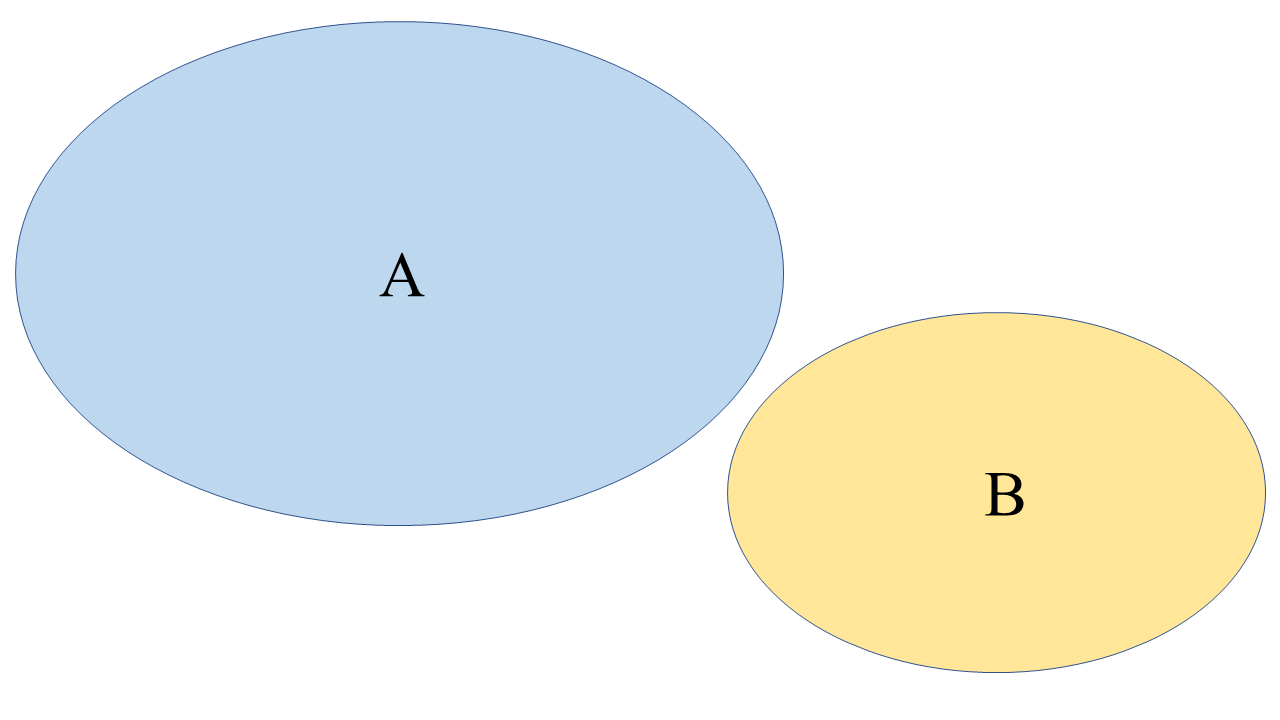
\includegraphics[width=0.7\textwidth]{graphics/mangButanformangdA.png}
 \end{center}
 
 Det minsta värdet $A \cup B$ kan anta är 15. I detta fallet (minsta möjliga unionen) kommer alla element i B vara närvarande i A. Alltså kommer vår nya mängd vara lika med mängden A, eftersom B också är närvarande i den mängden. 
 \begin{center}
    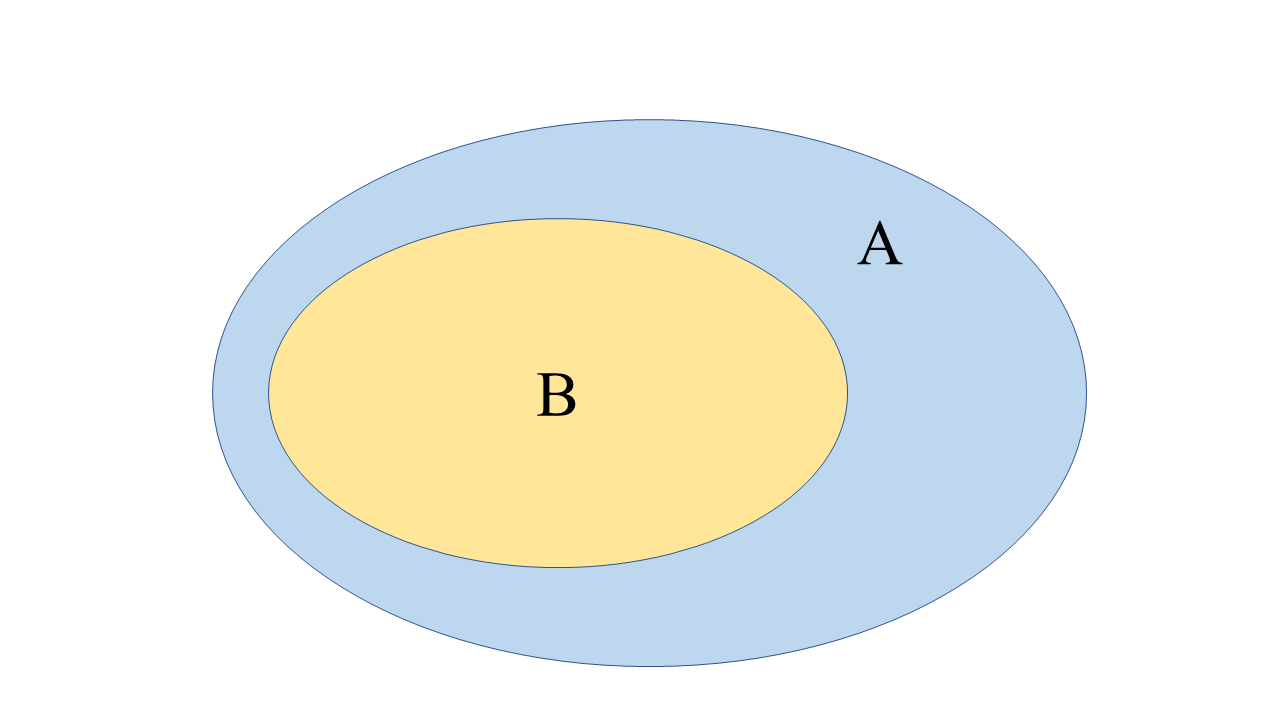
\includegraphics[width=0.7\textwidth]{graphics/mangimangdA.png}
 \end{center}

 \addlinespace

 6. Det största värdet som $A \cap B$ kan anta är 7. I detta faller kommer alla element i B vara närvarande i A. Då får vi vår nya mängd som innehåller alla element som finns i både A och i B. 
 Här kan vi visualisera problemet på samma sätt som andra bilden i övning 5.5 (bilden precis ovan).

 Det minsta värdet som $A \cap B$ kan anta är 0. I detta fallet så kommer alla element i B vara skilda från alla element i A och vårt snitt kommer då bli en tom mängd. 
 Här kan vi visualisera problemet på samma sätt som första bilden i övning 5.5 (två bilder upp).
\addlinespace

\noindent\textbf{Tips}

1. I sådana uppgifter är det bra att fundera över hur additionsregeln och multiplikationsregeln kan appliceras. 

2. Rita upp mängderna och de olika fallen, ligger mängderna i varandra (innehåller samma element), ligger de utanför varandra (innehåller inte samma element) eller ligger de delvis i varandra/utanförvarandra?

\end{xca}

\begin{xca}
	Du har sökt ett prestigefyllt internship, och ska klä dig för intervjun. Du inser att du borde ha slips på dig, och ser att du äger fem seriösa slipsar och sju slipsar med komiska tryck.
  
	Hur många sätt kan du välja slips för intervjun på?
  
	Efter lite eftertanke kommer du ihåg att jobbet du sökt är som clown,\sidenote[][-1cm]{Och tyvärr äger du ingen sådan där skoj fluga som kan spruta vatten i ansiktet på folk.}\sidenote[][]{Denna övningen är stulen från internet, och den handlade om en clownjobbintervju redan från början. Jag valde den helt baserat på hur mycket jag skrattade åt hur de antydde att deras studenter var clowner.} så du borde nog ha på dig två slipsar på samma gång, eftersom det är väldigt komiskt.

	På hur många sätt kan du välja två slipsar att ha på dig på samma gång? Hur många sätt kan du välja en seriös slips och en med ett komiskt tryck på?
  \end{xca}
  
  \noindent\textbf{Lösning}
    \newline a) Hur många sätt kan du välja slips för intervjun?
    \newline Additionsregeln ger att det finns 5+7 = 12 sätt att välja en slips att ha på sig på intervjun.
    \newline b) På hur många sätt kan du välja två slipsar att ha på dig på samma gång?
    Vi kan välja fritt mellan de seriösa slipsarna och de med komiskt tryck.
    Alltså hur många sätt kan man välja två slipsar från tolv stycken slipar.
    Det blir antalet kombinationer $$\binom{12}{2}$$
    \newline c) Hur många sätt kan du välja en seriös slips och en med ett komiskt tryck på?
    \newline Svaret ges av multiplikationsreglen, då vi vill veta hur många sätt vi kan välja en slips från mängden av seriösa slipsar och en slips från mängden av komiska slipsar.
    $$5\cdot 7 = 35$$

\bibliography{references}
\bibliographystyle{plainnat}



\end{document}
